You can automatically report the status of an automated test to an external system. The reporting is achieved by writing a comment on a task in the external repository. The comment includes a link to the test result in the dasboard. 

\subsubsection{Configuring a task repository for your \gdproject{}}
\label{TasksALMConfigureProject}
Once you have configured one or more repositories for your workspace \bxpref{TasksALMConfigureWorkspace}, you can select one of these to be the test-relevant repository for your \gdproject{}. 

This will let you:
\begin{itemize}
\item Add a task ID from this repository to \gdcases{} and \gdsuites{} in the \gdproject{} to signify that this item is the test for this task \bxpref{TasksALMAddTask}.
\item Automatically report test results to the task defined when a test runs.
\item View the test results for the relevant item in the dashboard as a link from the task repository.
\end{itemize}

\textbf{To configure a task repository for your \gdproject{}:}

\begin{enumerate}
\item In the \gdproject{} Properties, select \bxname{Mylyn ALM} from the tree on the left \bxfigref{TasksALMProjectProperties}.
\item In the page that appears, you can select a repository from the combo-box. You can validate the repository settings using the button.
\item You can then choose whether to only report failed tests, only report successful tests, or both.
\item Enter the URL of the \dash{} that is configured to use the correct \gddb{} for your test results. This is the \dash{} that will be opened when you click on a test result link from the task repository. For more information on configuring and starting the \dash{}, see the documentation \bxpref{TasksDashboard}.
\end{enumerate}

\begin{figure}[h]
\begin{center}
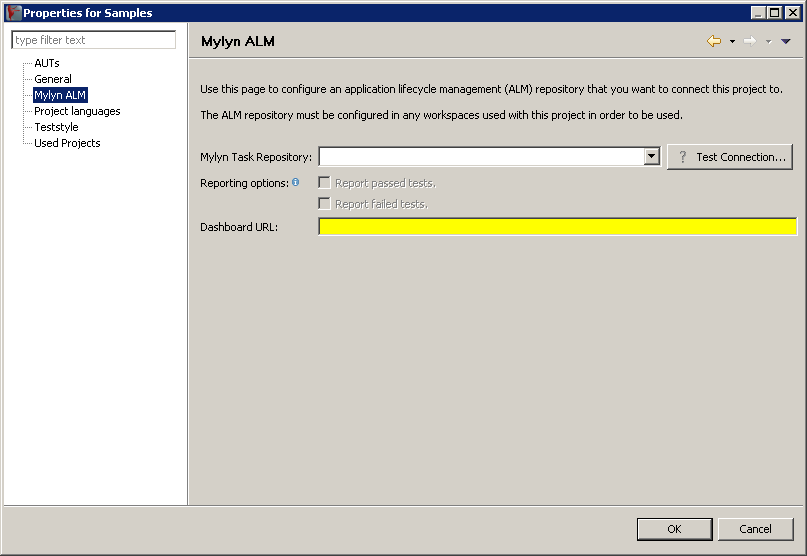
\includegraphics[width=12.5cm]{Tasks/ALM/PS/almproperties}
\caption{ALM Settings}
\label{TasksALMProjectProperties}
\end{center}
\end{figure}



\subsubsection{Adding task IDs to \gdsuites{} and \gdcases{}}
\label{TasksALMAddTask}

You can add a task ID to \gdcases{} and \gdsuites{} in your \gdproject{}. 

The task ID should be a valid ID in the repository that you have specified as the repository for this \gdproject{} \bxpref{TasksALMConfigureProject}. Adding the task ID to an item in your \gdproject{} means that this item is the relevant test for that task in your repository. You will be able to report test results for this item as a comment to the task in the repository. The comment will include a link to the dashboard, in which the test result report can be viewed.

To add a task ID to a \gdcase{} or \gdsuite{}:
\begin{enumerate}
\item Open the item in the editor by double-clicking it.
\item In the \gdpropview{}, in the cell for \bxname{Task ID}, enter the task ID from the external repository. You can only enter task IDs at the place of specification -- you cannot overwrite them when you reuse the item.
\item Save the editor. 
\item When you have added a task ID to a node, you can open the task for this node from the browser by selecting:\\
\bxmenu{Open with}{Mylyn Task Editor}{}
\end{enumerate}

\bxtipp{You should ensure that you add task IDs to the right node-level to provide you with the relevant amount of information for the tasks in your repository. This will usually be at the level of Use Cases within a \gdsuite{}. }

\subsubsection{Test execution with reporting to external repositories}
If your \gdproject{} is joined to an external repository \bxpref{TasksALMConfigureProject}, and you have added task IDs to one or more items in your \gdproject{} \bxpref{TasksALMAddTask}, then you will be able to report the test results to the repository after the test has run. The test run can be either via the \ite{} or via the command line \bxname{testexec}.  

\bxtipp{If you run a test via the \ite{} which should report to ALM systems, the reporting is triggered automatically once the test has run. If the reporting for the test run encounters an error, then you will be able to manually trigger the reporting later \bxpref{TasksALMReportTestExec}. To report to ALM systems after running a test via testexec, you must also  manually trigger the recording \bxpref{TasksALMReportTestExec}.}

When reporting is triggered, the following happens:
\begin{itemize}
\item A connection is made to ALM system configured in the \gdproject{} properties. 
\item The test results are then analyzed to see if any comments need to be added in the external repository (commenting can be (de)activated for failed nodes or successful nodes in the \gdproject{} properties, for example). 
\item If there are comments to be added, the \ite{} writes one comment per task, as defined in the \gdproject{} properties. If multiple items in one test run reference the same task ID, or if an item with a task ID is executed multiple times in the same test run,  then each test status and result link is written, but all in one comment. 
\bxtipp{Tests that have a status other than \bxname{passed} (e.g. failed, stopped, still testing) are considered as \bxname{failed}.}
\item You can see the status of the ALM reporting in the console view. 
\item Once a comment has been written, you can see the comment in the external repository. From there, you can click on the link provided to open the test result report in the \dash{} that you specified for your \gdproject{}. The \dash{} must be already running for this action to succeed. The test results must also still be present in the \gddb{} \bxpref{TasksReopenTestResult}.
\item The test result report is opened at the node which referenced the current task ID. 
\item You can see the status of the reporting in the \gdtestsummaryview{} \bxpref{TasksALMReportTestExec}.
\bxtipp{The integration for writing to external repositories can be used with Bugzilla 3.6+, JIRA 5.0+ and HP ALM 11+. Other repositories for which there are Mylyn connectors may also work, but these have not been tested.}
\end{itemize}

\textbf{Reporting to ALM repositories after a test started via testexec}
\label{TasksALMReportTestExec}
For tests started via testexec, the reporting does not happen automatically. Instead, you must choose to report to ALM from the \gdtestsummaryview{}.

\begin{enumerate}
\item In a \gdproject{} that is configured to report to an ALM repository, when a test has run via testexec, you can open the Reporting Perspective and locate the test run in the \gdtestsummaryview{}.
\item In the \bxname{ALM Report Status} column, you will see whether there are any reports pending. You can see various statuses in this column:

\begin{description}
\item [Not configured:]{if you have not configured ALM reporting for the \gdproject{}, or if the relevance of the test run was set to false when the test was started. This status will also be shown if you have exported the \gdproject{} and imported it -- no reporting data or statuses are transferred via export/import.}
\item [Not yet reported:]{if reporting was configured for the \gdproject{}, and there is information available to be reported that has not yet been reported, e.g. from a test run via testexec. You will also see this status if you have run a test via the \ite{} that could not report to the ALM system due to e.g. a connection problem. This allows you to report test results later, once the problem has been resolved.}
\item [Reported:]{this status will be shown if you have run a test with reporting configured via the \ite{}, which reports automatically. It will also be shown if you have chosen to report to the ALM system after running a test via testexec. This status will also be shown even if the test run was not linked to any tasks, but reporting is configured for the \gdproject{}. It can be understood as \bxname{any reporting that was necessary has been carried out}.}
\item [Report discarded:]{if reporting information was available, but the information was discarded and therefore not reported. You can do this by selecting the option to discard a pending report from the context menu.}
\item [Marked as non-relevant:]{you will see this status for any test runs that were marked as relevant when the test was started and which have information to report (status: \bxname{Not yet reported}),but which you then mark as non-relevant by toggling the relevance in the \gdtestsummaryview{}. This status means that you could report or discard the information, but only if you re-toggle the test run to be relevant.}
\end{description}
\item Select any test runs whose results you want to report to ALM, and click on the \bxcaption{Report to ALM} button on the toolbar. You can also select this option from the context-sensitive menu. If you select multiple test runs, the reporting will take place sequentially for each test run. 
\item When you select this option, the reporting will be triggered as described above. If the reporting is successful, the status in the \bxname{ALM Report Status} column changes from \bxname{Not yet reported} to \bxname{Reported}. If an error occurs, then the status remains as \bxname{Not yet reported}. 
\item If you do not want to report the test results to an ALM tool, you can discard the reporting information by selecting the option to discard a pending report from the context menu. This changes the status in the \bxname{ALM Report Status} column  from \bxname{Not yet reported} to \bxname{Report discarded}.
\end{enumerate}


\subsubsection{Specific information for HP ALM users}
\begin{itemize}
\item To use the HP ALM integration, you must use a separate connector for HP ALM which may incur license costs. Visit the Tasktop website for more details \url{http://www.tasktop.com}.
\item If you have changed the attribute IDs in your HP ALM installation for defects and / or requirements from their relative defaults (\bxname{BG\_DEV\_COMMENTS} and \bxname{REQ\_DEV\_COMMENTS}), or if you have changed the ID for the connector, then you must modify these properties in the \bxshell{almAccess.properties} file contained in the jar:\\
\bxname{org.eclipse.jubula.client.alm.mylyn.core} 
\item Since tasks in HP ALM only have one comment field, the result information is appended to the comment field instead of being added as a new comment each time.
\item To write to requirements in a default HP ALM installation, you must use the prefix \bxname{REQ}, e.g. REQ100. To write to defects in a default HP ALM installation, you must use the prefix \bxname{DEF}, e.g. DEF42.
\end{itemize}


